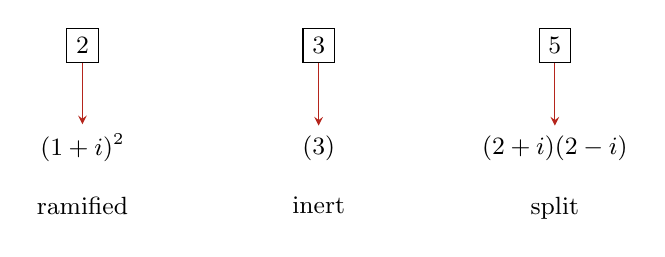
\begin{tikzpicture}[>=stealth,font=\small]
\node[draw] (a) at (0,0) {$2$}; \node[draw] (b) at (3,0) {$3$}; \node[draw] (c) at (6,0) {$5$};
\node (aa) at (0,-1.3) {$(1+i)^2$};\node (bb) at (3,-1.3) {$(3)$}; \node (cc) at (6,-1.3) {$(2+i)(2-i)$};
\draw[->,BrickRed] (a)--(aa);\draw[->,BrickRed] (b)--(bb);\draw[->,BrickRed] (c)--(cc);
\node[below] at (0,-1.8) {ramified};\node[below] at (3,-1.8) {inert};\node[below] at (6,-1.8) {split};
\end{tikzpicture}
